\documentclass[a5paper, 10pt]{article}

% Текст
\usepackage[utf8]{inputenc} % UTF-8 кодировка
\usepackage[russian]{babel} % Русский язык
\usepackage{indentfirst} % красная строка в первом параграфе в главе
% Отображение страниц
\usepackage{geometry} % размеры листа и отступов
\geometry{
	left=12mm,
	top=25mm,
	right=15mm,
	bottom=17mm,
	marginparsep=0mm,
	marginparwidth=0mm,
	headheight=10mm,
	headsep=7mm,
	nofoot}
\usepackage{afterpage,fancyhdr} % настройка колонтитулов
\pagestyle{fancy}
\fancypagestyle{style}{ % создание нового стиля style
	\fancyhf{} % очистка колонтитулов
	\fancyhead[LO, RE]{Лабораторная работа № 2 } % название документа наверху
	\fancyhead[RO, LE]{ 2D-преобразования } % название section наверху
	\fancyfoot[RO, LE]{\thepage} % номер страницы справа внизу на нечетных и слева внизу на четных
	\renewcommand{\headrulewidth}{0.25pt} % толщина линии сверху
	\renewcommand{\footrulewidth}{0pt} % толцина линии снизу
}
\fancypagestyle{plain}{ % создание нового стиля plain -- полностью пустого
	\fancyhf{}
	\renewcommand{\headrulewidth}{0pt}
}
\fancypagestyle{title}{ % создание нового стиля title -- для титульной страницы
	\fancyhf{}
	\fancyhead[C]{{\footnotesize
			Министерство образования и науки Российской Федерации\\
			Федеральное государственное автономное образовательное учреждение высшего образования
	}}
	\fancyfoot[C]{{\large 
			Санкт-Петербург, 2023-2024
	}}
	\renewcommand{\headrulewidth}{0pt}
}

% Математика
\usepackage{amsmath, amsfonts, amssymb, amsthm} % Набор пакетов для математических текстов
%\usepackage{dmvnbase} % мехматовский пакет latex-сокращений
\usepackage{cancel} % зачеркивание для сокращений
% Рисунки и фигуры
\usepackage[pdftex]{graphicx} % вставка рисунков
\usepackage{wrapfig, subcaption} % вставка фигур, обтекая текст
\usepackage{caption} % для настройки подписей
\captionsetup{figurewithin=none,labelsep=period, font={small,it}} % настройка подписей к рисункам
% Рисование
\usepackage{tikz} % рисование
\usepackage{circuitikz}
\usepackage{pgfplots} % графики
% Таблицы
\usepackage{multirow} % объединение строк
\usepackage{multicol} % объединение столбцов
% Остальное
\usepackage[unicode, pdftex]{hyperref} % гиперссылки
\usepackage{enumitem} % нормальное оформление списков
\setlist{itemsep=0.15cm,topsep=0.15cm,parsep=1pt} % настройки списков
% Теоремы, леммы, определения...
\theoremstyle{definition}
\newtheorem{Def}{Определение}
\newtheorem*{Axiom}{Аксиома}
\theoremstyle{plain}
\newtheorem{Th}{Теорема}
\newtheorem{Lem}{Лемма}
\newtheorem{Cor}{Следствие}
\newtheorem{Ex}{Пример}
\theoremstyle{remark}
\newtheorem*{Note}{Замечание}
\newtheorem*{Solution}{Решение}
\newtheorem*{Proof}{Доказательство}
% Свои команды
\newcommand{\comb}[1]{\left[\hspace{-4pt}\begin{array}{l}#1\end{array}\right.\hspace{-5pt} } % совокупность уравнений
% Титульный лист
\usepackage{csvsimple-l3}
\newcommand*{\titlePage}{
	\thispagestyle{title}
	\begingroup
	\begin{center}
		%		{\footnotesize
			%			Министерство образования и науки Российской Федерации\\
			%			Федеральное государственное автономное образовательное учреждение высшего образования
			%		}
		%		
		\vspace*{6ex}
		
		{\small
			САНКТ-ПЕТЕРБУРГСКИЙ НАЦИОНАЛЬНЫЙ ИССЛЕДОВАТЕЛЬСКИЙ УНИВЕРСИТЕТ ИТМО	
		}
		
		\vspace*{2ex}
		
		{\normalsize
			Факультет систем управления и робототехники
		}
		
		\vspace*{15ex}
		
		{\Large \bfseries 
			Лабораторная работа № 2
		}
\vspace*{2ex}
	{\Large \bfseries 
			
"2D-преобразования "
		}
\vspace*{2ex}
		
		{\normalsize
			по дисциплине Практическая линейная алгебра
		}

	\end{center}
	\vspace*{20ex}
	\begin{flushright}
		{\large 
			\underline{Выполнила}: студентка гр. \textbf{R3238}\\
			\begin{flushright}
				\textbf{Нечаева А. А.}\\
			\end{flushright}
		}
		
		\vspace*{5ex}
		
		{\large 
			\underline{Преподаватель}: \textit{Перегудин Алексей Алексеевич}
		}
	\end{flushright}	
	\newpage
	\setcounter{page}{1}
	\endgroup}

\begin{document}
	\titlePage
	\pagestyle{style}
\newpage

Перед началом выполнения работы выберем 4 различных числа: $$a = 2$$ $$b = 8$$ $$c = 5$$ $$d=3$$
Отображение имеет вид:
\begin{equation}
\begin{bmatrix}
x_{new}\\
y_{new}
\end{bmatrix}
=
\begin{bmatrix}
* & *\\
* & *
\end{bmatrix}
\begin{bmatrix}
x_{old}\\
y_{old}
\end{bmatrix}
\end{equation}


\section{Задание.}
 Придумать матрицы $2 \times 2$, которые задают:
\subsection{}
\textit{Отражение (симметрию) плоскости относительно прямой $y=ax$, в нашем случае после подстановки $a=2$, получаем $y=2x$. Задача -- найти матрицу вида}:
\begin{equation}
\begin{bmatrix}
m_{0 0} & m_{0 1}\\
m_{1 0} & m_{1 1}
\end{bmatrix}
\end{equation}
Рассмотрим отражение 2 точек плоскости относительно прямой  $y=2x$.\\
Для точки $A (2; 2)$:
\begin{equation}
\begin{bmatrix}
m_{0 0} & m_{0 1}\\
m_{1 0} & m_{1 1}
\end{bmatrix}
\begin{bmatrix}
2\\
2
\end{bmatrix}
=
\begin{bmatrix}
0.4\\
2.8
\end{bmatrix}
\to
\begin{cases}
2(m_{0 0} +  m_{0 1}) = 0.4\\
2(m_{1 0} + m_{1 1}) = 2.8
\end{cases}
\end{equation}
И, соотвественно, для точки $B(1;2)$:
\begin{equation}
\begin{bmatrix}
m_{0 0} & m_{0 1}\\
m_{1 0} & m_{1 1}
\end{bmatrix}
\begin{bmatrix}
1\\
2
\end{bmatrix}
=
\begin{bmatrix}
1\\
2
\end{bmatrix}
\to
\begin{cases}
m_{0 0} +  2m_{0 1} = 1\\
m_{1 0} + 2m_{1 1} = 2
\end{cases}
\end{equation}
Объединим, системы уравнений:
\begin{equation}
\begin{cases}
2(m_{0 0} +  m_{0 1}) = 0.4\\
2(m_{1 0} + m_{1 1}) = 2.8\\
m_{0 0} +  2m_{0 1} = 1\\
m_{1 0} + 2m_{1 1} = 2
\end{cases}
\end{equation}
И получим ответ:
\begin{equation}
\begin{cases}
m_{0 0} = -0.6\\
m_{0 1} = 0.8\\
m_{1 0} = 0.8\\
m_{1 1} = 0.6
\end{cases}
\end{equation}
\textit{\textbf{Искомая матрица}}:
\begin{equation}
\begin{bmatrix}
-0.6 & 0.8\\
0.8 & 0.6
\end{bmatrix}
\end{equation}

\subsection{}
\textit{Отображение всей плоскости в прямую $y=bx$  $(y=8x)$.}
Предположим, что все точки плоскости сохраняют координату $x$ и меняют только координату $y$ по закону $y=8x$. Рассмотрим также преобразование для двух точек.\\
Для точки $A (1; 5)$:
\begin{equation}
\begin{bmatrix}
m_{0 0} & m_{0 1}\\
m_{1 0} & m_{1 1}
\end{bmatrix}
\begin{bmatrix}
1\\
5
\end{bmatrix}
=
\begin{bmatrix}
1\\
8
\end{bmatrix}
\to
\begin{cases}
m_{0 0} +  5m_{0 1} = 1\\
m_{1 0} + 5 m_{1 1} = 8
\end{cases}
\end{equation}
И, соотвественно, для точки $B(3;7)$:
\begin{equation}
\begin{bmatrix}
m_{0 0} & m_{0 1}\\
m_{1 0} & m_{1 1}
\end{bmatrix}
\begin{bmatrix}
3\\
7
\end{bmatrix}
=
\begin{bmatrix}
3\\
24
\end{bmatrix}
\to
\begin{cases}
3m_{0 0} +  7m_{0 1} = 3\\
3m_{1 0} + 7m_{1 1} = 24
\end{cases}
\end{equation}
Заметим, что решением будет: 
\begin{equation}
\begin{cases}
m_{0 0} = 1\\
m_{0 1} = 0\\
m_{1 0} = 8\\
m_{1 1} = 0
\end{cases}
\end{equation}
\textit{\textbf{Искомая матрица}}:
\begin{equation}
\begin{bmatrix}
1 & 0\\
8 & 0
\end{bmatrix}
\end{equation}

\newpage
\subsection{}
\textit{Поворот плоскости на $10 * 5 = 50$ градусов против часовой стрелки.}
Запишем матрицу поворота при движении по часовой стрелке на угол $\phi$:
\begin{equation}
\begin{bmatrix}
\cos \phi & \sin \phi \\
-\sin \phi & \cos \phi
\end{bmatrix}
\end{equation}
И преобразуем матрицу для поворота против часовой стрелки (на угол $-\phi$):
\begin{equation}
\begin{bmatrix}
\cos \phi & -\sin \phi \\
\sin \phi & \cos \phi
\end{bmatrix}
\end{equation}
Перед подстановкой угла, запишем преобразование его из градусов в радианы:
\begin{equation}
\phi = \frac{50\pi}{180} =  \frac{5\pi}{18}
\end{equation}
\textit{\textbf{Искомая матрица}}:
\begin{equation}
\begin{bmatrix}
\cos  \frac{5\pi}{18} & -\sin  \frac{5\pi}{18} \\
\\
\sin  \frac{5\pi}{18} & \cos  \frac{5\pi}{18}
\end{bmatrix}
\end{equation}

\subsection{}
\textit{Центральную симметрию плоскости относительно начала координат}
Матрица, заадющая центральную симметрию:
\begin{equation}
\begin{bmatrix}
-1 & 0\\
0 & -1
\end{bmatrix}
\end{equation}
Убедимся в этом на примере точки $A(2; 3)$:
\begin{equation}
\begin{bmatrix}
-1 & 0\\
0 & -1
\end{bmatrix}
\begin{bmatrix}
2\\
3
\end{bmatrix}
=
\begin{bmatrix}
-2\\
-3
\end{bmatrix}
\end{equation}
\textit{\textbf{Искомая матрица}}:
\begin{equation}
\begin{bmatrix}
-1 & 0\\
0 & -1
\end{bmatrix}
\end{equation}

\newpage
\subsection{}
\textit{Отображение, которое можно описать так: сначала отражение относительно прямой $y=2x$, потом поворот на 30 градусов по часовой стрелке.}
\\Пусть $A$ -- матрица отражения относительно прямой  $y=2x$, $B$ -- матрица поворота на 30 градусов по часовой стрелке, $C_{old}$, $C_{new}$ -- матрицы координат до преобразования и после соотвественно. Запишем необходимое преобразование координат:

\begin{equation}
B(AC_{old}) = C_{new}
\end{equation}
Воспользуемся свойством ассоциативности умножения матриц:
\begin{equation}
(BA)C_{old} = C_{new}
\end{equation}
Согласно п. 1.1 матрица $A$:
\begin{equation}
\begin{bmatrix}
-0.6 & 0.8\\
0.8 & 0.6
\end{bmatrix}
\end{equation}
Найдем матрицу $B$, подставив в выражение (12) из пункта 1.3 $\phi = \frac{\pi}{6}$:
\begin{equation}
B = 
\begin{bmatrix}
\cos \frac{\pi}{6} & \sin \frac{\pi}{6} \\
\\
-\sin \frac{\pi}{6} & \cos \frac{\pi}{6}
\end{bmatrix}
\end{equation}
Перемножим матрицы $B$ и $A$:

\begin{equation}
BA =
\begin{bmatrix}
\frac{\sqrt{3}}{2} &  \frac{1}{2} \\
\\
- \frac{1}{2} & \frac{\sqrt{3}}{2}
\end{bmatrix}
\begin{bmatrix}
-0.6 & 0.8\\
0.8 & 0.6
\end{bmatrix}
=
\begin{bmatrix}
-0.3\sqrt{3} + 0.4 & 0.4\sqrt{3} + 0.3\\
0.3 + 0.4\sqrt{3} & -0.4 + 0.3\sqrt{3}
\end{bmatrix}
\end{equation}

\textit{\textbf{Искомая матрица}}:
\begin{equation}
\begin{bmatrix}
-0.3\sqrt{3} + 0.4 & 0.4\sqrt{3} + 0.3\\
0.3 + 0.4\sqrt{3} & -0.4 + 0.3\sqrt{3}
\end{bmatrix}
\end{equation}

\newpage
\subsection{}
\textit{Отображение, которое переводит прямую $y=0$ в $y=2x$ и прямую $x=0$ в $y=8x$}\\
Пусть $A$ -- матрица, переводящая прямую $y=0$ в $y=2x$:
\begin{equation}
A=
\begin{bmatrix}
1 & 0\\
2 & 0
\end{bmatrix}
\end{equation}
$B$ -- матрица, переводящая прямую $x=0$ в $y=8x$:
\begin{equation}
B=
\begin{bmatrix}
0 & \frac{1}{8}\\
0 & 1
\end{bmatrix}
\end{equation}
\textit{\textbf{Искомая матрица}}:
\begin{equation}
\begin{bmatrix}
1 &  \frac{1}{8}\\
2 & 1
\end{bmatrix}
\end{equation}


\subsection{}
\textit{Отображение, которое переводит прямую $y=2x$ в $y=0$  и прямую $y=8x$ в $x=0$}\\
Так как преобразование -- обратное, проводимому в пункте 1.6. Матрицу можно найти, вычислив обратную.
\begin{equation}
M = 
\begin{bmatrix}
1 &  \frac{1}{8}\\
2 & 1
\end{bmatrix}^{-1}
=
\frac{4}{3} 
\begin{bmatrix}
1 &  -\frac{1}{8}\\
-2 & 1
\end{bmatrix}
\end{equation}

\textit{\textbf{Искомая матрица}}:
\begin{equation}
\frac{4}{3}
\begin{bmatrix}
1 &  -\frac{1}{8}\\
-2 & 1
\end{bmatrix}
\end{equation}


\subsection{}
\textit{Отображение, которое меняет местами $y=2x$ и $y=8x$.}\\
Пусть $M$ -- искомая матрица. Запишем 2 преобразования:

\begin{equation}
\begin{bmatrix}
m_{0 0} & m_{0 1}\\
m_{1 0} & m_{1 1}
\end{bmatrix}
\begin{bmatrix}
2\\
4
\end{bmatrix}
=
\begin{bmatrix}
2\\
16
\end{bmatrix}
\to
\begin{cases}
2m_{0 0} + 4m_{0 1} = 2\\
2m_{1 0} + 4m_{1 1} = 16
\end{cases}
\end{equation}

\begin{equation}
\begin{bmatrix}
m_{0 0} & m_{0 1}\\
m_{1 0} & m_{1 1}
\end{bmatrix}
\begin{bmatrix}
3\\
24
\end{bmatrix}
=
\begin{bmatrix}
3\\
6
\end{bmatrix}
\to
\begin{cases}
3m_{0 0} + 24m_{0 1} = 3\\
3m_{1 0} + 24m_{1 1} = 6
\end{cases}
\end{equation}
Пусть $ m_{0 0} = 1$ , $m_{0 1} = 0$. Решим систему, чтобы найти оставшиеся компоненты:
\begin{equation}
\begin{cases}
2m_{1 0} + 4m_{1 1} = 16\\
3m_{1 0} + 24m_{1 1} = 6
\end{cases}
\to
\begin{cases}
m_{1 0} = 10\\
m_{1 1} = -1
\end{cases}
\end{equation}
\textit{\textbf{Искомая матрица}}:
\begin{equation}
\begin{bmatrix}
1 &  0\\
10 & -1
\end{bmatrix}
\end{equation}

\subsection{}
\textit{Отображение, которое переводит круг единичной площади с центром в начале координат в круг площади $c=5$.}\\
Определитель матрицы преобразования -- множитель площади, то есть в нашем случае определитель искомой матрицы равен 5. \\
\begin{equation}
\begin{bmatrix}
\sqrt{5} & 0\\
0 & \sqrt{5}
\end{bmatrix}
\end{equation}
\textit{\textbf{Искомая матрица}}:
\begin{equation}
\begin{bmatrix}
\sqrt{5} & 0\\
0 & \sqrt{5}
\end{bmatrix}
\end{equation}


\subsection{}
\textit{Отображение, которое переводит круг единичной площади с центром в начале координат в некруг площади $d=3$.}\\
Определитель матрицы преобразования -- множитель площади, то есть в нашем случае определитель искомой матрицы равен 3. \\
\textit{\textbf{Искомая матрица}}:
\begin{equation}
\begin{bmatrix}
3 & 0\\
0 & 1
\end{bmatrix}
\end{equation}

\subsection{}
\textit{Отображение, у которого собственные вектора перпендикулярны, и ни один из них не лежит на прямой $y=0$ или $y=x$.}\\
Пусть собственные векторы:
\begin{equation}
v_1 = 
\begin{bmatrix}
1\\
2
\end{bmatrix}
,
v_2 = 
\begin{bmatrix}
-6\\
3
\end{bmatrix}
\end{equation}
И собственные числа, соотвествующие им $\lambda_1 = 2$ и $\lambda_2 = 1$. По этим данным восстановим матрицу отображения $M$:
\begin{equation}
\begin{bmatrix}
m_{0 0} & m_{0 1}\\
m_{1 0} & m_{1 1}
\end{bmatrix}
\begin{bmatrix}
1\\
2
\end{bmatrix}
=
\begin{bmatrix}
2\\
4
\end{bmatrix}
\to
\begin{cases}
m_{0 0} + 2m_{0 1} = 2\\
m_{1 0} + 2m_{1 1} = 4
\end{cases}
\end{equation}

\begin{equation}
\begin{bmatrix}
m_{0 0} & m_{0 1}\\
m_{1 0} & m_{1 1}
\end{bmatrix}
\begin{bmatrix}
-6\\
3
\end{bmatrix}
=
\begin{bmatrix}
-6\\
3
\end{bmatrix}
\to
\begin{cases}
-6 m_{0 0} + 3m_{0 1} = -6\\
-6m_{1 0} + 3m_{1 1} = 3
\end{cases}
\to
\begin{cases}
2 m_{0 0} - m_{0 1} = 2\\
2m_{1 0} - m_{1 1} = -1
\end{cases}
\end{equation}

\begin{equation}
\begin{cases}
m_{0 0} + 2m_{0 1} = 2\\
m_{1 0} + 2m_{1 1} = 4\\
2 m_{0 0} - 2 =  m_{0 1}\\
2m_{1 0} + 1 = m_{1 1} 
\end{cases}
\to
\begin{cases}
m_{0 0} = \frac{6}{5}\\
m_{1 0}  = \frac{2}{5}\\
m_{0 1} = \frac{2}{5} \\
m_{1 1} = \frac{9}{5}
\end{cases}
\end{equation}

\textit{\textbf{Искомая матрица}}:
\begin{equation}
\begin{bmatrix}
 \frac{6}{5} & \frac{2}{5}\\
\\
\frac{2}{5} &  \frac{9}{5}
\end{bmatrix}
\end{equation}

\subsection{}
\textit{Отображение, у которого нет двух неколлинеарных собственных векторов.}\\
Пусть задана матрица:
\begin{equation}
M = 
\begin{bmatrix}
4 & 1\\
0 & 4
\end{bmatrix}
\end{equation}
Найдем ее собственные числа: $\lambda_1 = 4$ и $\lambda_2 = 4$ . Соответствующие собственные векторы: $\begin{bmatrix}
a\\
0 
\end{bmatrix}$ и $\begin{bmatrix}
b\\
0  
\end{bmatrix}$, где $a, \, b \in \mathbb {R}$. Такие векторы всегда будут коллинеарны.\\
\\
\textit{\textbf{Искомая матрица}}:
\begin{equation}
\begin{bmatrix}
4 & 1\\
0 & 4
\end{bmatrix}
\end{equation}


\newpage
\subsection{}
\textit{Отображение, у которого нет ни одного вещественного собственного вектора (но при этом само отображение задается вещественной матрицей).}\\
\begin{equation}
M =
\begin{bmatrix}
0 & -1\\
4 & 0
\end{bmatrix}
\end{equation}
Собственные числа и соотвествующие им собственные вектры:
\begin{equation}
\lambda_1 = 2i, \, \, 
v_1 = 
\begin{bmatrix}
\frac{i}{2}\\
1
\end{bmatrix}
,
\lambda_2 =- 2i, \, \, 
v_2 = 
\begin{bmatrix}
-\frac{i}{2}\\
1
\end{bmatrix}
\end{equation}

\textit{\textbf{Искомая матрица}}:
\begin{equation}
\begin{bmatrix}
0 & -1\\
4 & 0
\end{bmatrix}
\end{equation}


\subsection{}
\textit{Отображение, для которого любой ненулевой вектор является собственным.}\\

\textit{\textbf{Искомая матрица}}:
\begin{equation}
\begin{bmatrix}
0 & 0\\
0 & 0
\end{bmatrix}
\end{equation}


\subsection{}
\textit{Пару отображений, последовательное применение которых дает различные результаты в зависимости от порядка $AB \neq BA$.}\\

\textit{\textbf{Искомые матрицы}}:
\begin{equation}
A=
\begin{bmatrix}
1 & 2\\
3 & 4
\end{bmatrix}
, \, \, \, 
B=
\begin{bmatrix}
5 & 6\\
7 & 8
\end{bmatrix}
\end{equation}

\newpage
\subsection{}
\textit{Пару отображений, последовательное применение которых дает одинаковый результат независимо от порядка $AB = BA$.}\\
Пусть матрица $A$:

\begin{equation}
A=
\begin{bmatrix}
1 & 4\\
0 & 2
\end{bmatrix}
\end{equation}
Найдем какую-нибудь коммутативную к ней матрицу $B$:
\begin{equation}
B=
\begin{bmatrix}
b_{0 0} & b_{0 1}\\
b_{1 0} & b_{1 1}
\end{bmatrix}
\end{equation}
\begin{equation}
AB= BA \to
\begin{bmatrix}
1 & 4\\
0 & 2
\end{bmatrix}
\begin{bmatrix}
b_{0 0} & b_{0 1}\\
b_{1 0} & b_{1 1}
\end{bmatrix}
=
\begin{bmatrix}
b_{0 0} & b_{0 1}\\
b_{1 0} & b_{1 1}
\end{bmatrix}
\begin{bmatrix}
1 & 4\\
0 & 2
\end{bmatrix}
\end{equation}

\begin{equation}
\begin{cases}
b_{0 0} + 4b_{1 0} = b_{0 0}\\
b_{0 1} + 4 b_{1 1} = 4b_{0 0} + 2b_{0 1}\\
2b_{1 0} = b_{1 0}\\
2 b_{1 1} = 2b_{1 1}
\end{cases}
\to
\begin{cases}
b_{1 0} = 0\\
b_{0 0} = b_{0 0}\\
b_{0 1} + 4 b_{1 1} = 4b_{0 0} + 2b_{0 1}\\
2 b_{1 1} = 2b_{1 1}
\end{cases}
\end{equation}
Пусть $b_{0 0} = 9$ и $b_{1 1} = 11$

\begin{equation}
\begin{cases}
b_{1 0} = 0\\
b_{0 0} = 9\\
b_{0 1} + 4 b_{1 1} = 4b_{0 0} + 2b_{0 1}\\
 b_{1 1} = 11
\end{cases}
\to
\begin{cases}
b_{1 0} = 0\\
b_{0 0} = 9\\
b_{0 1} = 8\\
 b_{1 1} = 11
\end{cases}
\end{equation}


\textit{\textbf{Искомые матрицы}}:
\begin{equation}
A=
\begin{bmatrix}
1 & 4\\
0 & 2
\end{bmatrix}
, \, \, \, 
B=
\begin{bmatrix}
9 & 8\\
0 & 11
\end{bmatrix}
\end{equation}


\newpage
\section{Анализ}
\subsection{}
\textit{Найти образ и ядро придуманных отображений из пунктов 1, 2, 13, 14.}\\
\\
Для пункта 1:
\begin{equation}
A =
\begin{bmatrix}
-0.6 & 0.8\\
0.8 & 0.6
\end{bmatrix}
\end{equation}
Найдем образ, для этого приведем матрицу к приведённому ступенчатому виду:
\begin{equation}
\begin{bmatrix}
-0.6 & 0.8\\
0.8 & 0.6
\end{bmatrix}
\to
\begin{bmatrix}
0.2 & 1.4\\
0.8 & 0.6
\end{bmatrix}
\to
\begin{bmatrix}
1 & 7\\
4 & 3
\end{bmatrix}
\to
\begin{bmatrix}
1 & 7\\
0 & -25
\end{bmatrix}
\to
\begin{bmatrix}
1 & 0\\
0 & 1
\end{bmatrix}
\end{equation}

\begin{equation}
Range(A) = Span
\left\{\
\begin{bmatrix}
-0.6\\
0.8
\end{bmatrix}
,
\begin{bmatrix}
0.8\\
0.6
\end{bmatrix}
\right\}\
\end{equation}

Найдем ядро отображения -- множество векторов, отображающихся в ноль:
\begin{equation}
\begin{bmatrix}
-0.6 & 0.8\\
0.8 & 0.6
\end{bmatrix}
\begin{bmatrix}
x_1\\
x_2
\end{bmatrix}
=
\begin{bmatrix}
0\\
0
\end{bmatrix}
\end{equation}

\begin{equation}
\begin{bmatrix}
-0.6 & 0.8 & | & 0\\
0.8 & 0.6 & | & 0
\end{bmatrix}
\to
\begin{bmatrix}
1 & 7 & | & 0\\
0 & -25 & | & 0
\end{bmatrix}
\to
\begin{cases}
x_1 = 0\\
x_2 = 0
\end{cases}
\end{equation}

\begin{equation}
Nullspace (A) = \varnothing
\end{equation}







Для пункта 2:
\begin{equation}
B =
\begin{bmatrix}
1 & 0\\
8 & 0
\end{bmatrix}
\end{equation}

Найдем образ, для этого приведем матрицу к приведённому ступенчатому виду:
\begin{equation}
\begin{bmatrix}
1 & 0\\
8 & 0
\end{bmatrix}
\to
\begin{bmatrix}
1 & 0\\
0 & 0
\end{bmatrix}
\end{equation}

\begin{equation}
Range(B) =  Span
\left\{\
\begin{bmatrix}
1\\
8
\end{bmatrix}
\right\}\
\end{equation}

Найдем ядро отображения -- множество векторов, отображающихся в ноль:
\begin{equation}
\begin{bmatrix}
1 & 0\\
8 & 0
\end{bmatrix}
\begin{bmatrix}
x_1\\
x_2
\end{bmatrix}
=
\begin{bmatrix}
0\\
0
\end{bmatrix}
\end{equation}

\begin{equation}
\begin{bmatrix}
1 & 0 & | & 0\\
8 & 0 & | & 0
\end{bmatrix}
\to
\begin{cases}
x_1 = 0\\
x_2 = x_2
\end{cases}
\end{equation}

\begin{equation}
Nullspace (B) = Span
\left\{\
\begin{bmatrix}
0\\
1
\end{bmatrix}
\right\}\
\end{equation}



Для пункта 13:
\begin{equation}
C =
\begin{bmatrix}
0 & -1\\
4 & 0
\end{bmatrix}
\end{equation}


Найдем образ, для этого приведем матрицу к приведённому ступенчатому виду:
\begin{equation}
\begin{bmatrix}
1 & 0\\
0 & 1
\end{bmatrix}
\end{equation}

\begin{equation}
Range(C) = Span
\left\{\
\begin{bmatrix}
0\\
4
\end{bmatrix}
,
\begin{bmatrix}
-1\\
0
\end{bmatrix}
\right\}\
\end{equation}

Найдем ядро отображения -- множество векторов, отображающихся в ноль:
\begin{equation}
\begin{bmatrix}
0 & -1\\
4 & 0
\end{bmatrix}
\begin{bmatrix}
x_1\\
x_2
\end{bmatrix}
=
\begin{bmatrix}
0\\
0
\end{bmatrix}
\end{equation}

\begin{equation}
\begin{bmatrix}
0 & -1 & | & 0\\
4 & 0 & | & 0
\end{bmatrix}
\to
\begin{cases}
x_1 = 0\\
x_2 = 0
\end{cases}
\end{equation}

\begin{equation}
Nullspace (С) = \varnothing
\end{equation}


Для пункта 14:
\begin{equation}
D =
\begin{bmatrix}
0 & 0\\
0 & 0
\end{bmatrix}
\end{equation}


Найдем образ, для этого приведем матрицу к приведённому ступенчатому виду:
\begin{equation}
\begin{bmatrix}
0 & 0\\
0 & 0
\end{bmatrix}
\end{equation}

\begin{equation}
Range(D) = \varnothing
\end{equation}

Найдем ядро отображения -- множество векторов, отображающихся в ноль:
\begin{equation}
\begin{bmatrix}
0 & 0\\
0 & 0
\end{bmatrix}
\begin{bmatrix}
x_1\\
x_2
\end{bmatrix}
=
\begin{bmatrix}
0\\
0
\end{bmatrix}
\end{equation}

\begin{equation}
\begin{bmatrix}
0 & 0 & | & 0\\
0 & 0 & | & 0
\end{bmatrix}
\to
\begin{cases}
x_1 = x_1\\
x_2 = x_2
\end{cases}
\end{equation}

\begin{equation}
Nullspace (D) = Span
 \left\{\
\begin{bmatrix}
a\\
b
\end{bmatrix}
,
\begin{bmatrix}
c\\
d
\end{bmatrix}
\right\}\
, \,\,  a, \, b, \, c, \, d \in \mathbb{R}
\end{equation}



\subsection{}
\textit{Найти собственные числа и собственные векторы придуманных отображений из пунктов 1, 2, 3, 4, 8, 11, 12, 13, 14, 15, 16.}\\
\\
Для пункта 1:
\begin{equation}
A =
\begin{bmatrix}
-0.6 & 0.8\\
0.8 & 0.6
\end{bmatrix}
\end{equation}
\begin{equation}
det(A - \lambda E) =
\begin{vmatrix}
-0.6 - \lambda & 0.8\\
0.8 & 0.6 - \lambda
\end{vmatrix}
 = \lambda^2 - 1 = 0 \, \, \to \lambda_1 = 1, \, \, \lambda_2 = -1
\end{equation}

Найдем собственный вектор, соответствующий $\lambda_1 = 1$:
\begin{equation}
\begin{bmatrix}
-0.6 & 0.8\\
0.8 & 0.6
\end{bmatrix}
\begin{bmatrix}
x_1 \\
x_2
\end{bmatrix}
=
\begin{bmatrix}
x_1 \\
x_2
\end{bmatrix}
\, \, \to 
\begin{cases}
x_1 = \frac{1}{2} \\
x_2 = 1
\end{cases}
\end{equation}

Найдем собственный вектор, соответствующий $\lambda_2 = -1$:
\begin{equation}
\begin{bmatrix}
-0.6 & 0.8\\
0.8 & 0.6
\end{bmatrix}
\begin{bmatrix}
x_1 \\
x_2
\end{bmatrix}
=
\begin{bmatrix}
x_1 \\
x_2
\end{bmatrix}
\, \, \to 
\begin{cases}
x_1 = 2 \\
x_2 = 1
\end{cases}
\end{equation}

Аналогично найдем собственные числа  и собственные векторы для остальных отображений.\\
\\
Для пункта 2:
\begin{equation}
B =
\begin{bmatrix}
1 & 0\\
8 & 0
\end{bmatrix}
\end{equation}
\begin{equation}
\lambda_1 = 0, \, \,
v_1 =
\begin{bmatrix}
0\\
1
\end{bmatrix}
, \, \,
\lambda_2 = 1, \, \,
v_2 =
\begin{bmatrix}
\frac{1}{8}\\
1
\end{bmatrix}
\end{equation}
\\

Для пункта 3:
\begin{equation}
C =
\begin{bmatrix}
\cos \frac{5\pi}{18} & -\sin \frac{5\pi}{18}\\
\\
\sin \frac{5\pi}{18} & \cos \frac{5\pi}{18}
\end{bmatrix}
\end{equation}
\begin{equation}
\lambda_1 \approx 0.643 - i 0.766, \, \,
v_1 =
\begin{bmatrix}
-i\\
1
\end{bmatrix}
, \, \,
\lambda_2 \approx 0.643 + i 0.766, \, \,
v_2 =
\begin{bmatrix}
i\\
1
\end{bmatrix}
\end{equation}
\\

Для пункта 4:
\begin{equation}
D =
\begin{bmatrix}
-1 & 0\\
0 & -1
\end{bmatrix}
\end{equation}
\begin{equation}
\lambda_1 = -1, \, \,
v_1 =
\begin{bmatrix}
1\\
0
\end{bmatrix}
, \, \,
\lambda_2 =  -1, \, \,
v_2 =
\begin{bmatrix}
0\\
1
\end{bmatrix}
\end{equation}
\\

Для пункта 8:
\begin{equation}
F =
\begin{bmatrix}
1 & 0\\
10 & -1
\end{bmatrix}
\end{equation}
\begin{equation}
\lambda_1 = 1, \, \,
v_1 =
\begin{bmatrix}
\frac{1}{5}\\
1
\end{bmatrix}
, \, \,
\lambda_2 =  -1, \, \,
v_2 =
\begin{bmatrix}
0\\
1
\end{bmatrix}
\end{equation}
\\

Для пункта 11:
\begin{equation}
G =
\begin{bmatrix}
\frac{6}{5} & \frac{2}{5}\\
\\
\frac{2}{5} & \frac{9}{5}
\end{bmatrix}
\end{equation}
\begin{equation}
\lambda_1 = 1, \, \,
v_1 =
\begin{bmatrix}
-2\\
1
\end{bmatrix}
, \, \,
\lambda_2 =  2, \, \,
v_2 =
\begin{bmatrix}
\frac{1}{2}\\
1
\end{bmatrix}
\end{equation}
\\

Для пункта 12:
\begin{equation}
H =
\begin{bmatrix}
4 & 1\\
0 & 4
\end{bmatrix}
\end{equation}
\begin{equation}
\lambda_1 = 4, \, \,
v_1 =
\begin{bmatrix}
1\\
0
\end{bmatrix}
, \, \,
\lambda_2 =  4, \, \,
v_2 =
\begin{bmatrix}
1\\
0
\end{bmatrix}
\end{equation}
\\

Для пункта 13:
\begin{equation}
K =
\begin{bmatrix}
0 & -1\\
4 & 0
\end{bmatrix}
\end{equation}
\begin{equation}
\lambda_1 = 2i, \, \,
v_1 =
\begin{bmatrix}
\frac{i}{2}\\
1
\end{bmatrix}
, \, \,
\lambda_2 =  -2i, \, \,
v_2 =
\begin{bmatrix}
-\frac{i}{2}\\
1
\end{bmatrix}
\end{equation}
\\

Для пункта 14:
\begin{equation}
L =
\begin{bmatrix}
0 & 0\\
0 & 0
\end{bmatrix}
\end{equation}
\begin{equation}
\lambda_1 = 0, \, \,
v_1 =
\begin{bmatrix}
1\\
0
\end{bmatrix}
, \, \,
\lambda_2 =  0, \, \,
v_2 =
\begin{bmatrix}
0\\
1
\end{bmatrix}
\end{equation}
\\

Для пункта 15:
\begin{equation}
M_1 =
\begin{bmatrix}
1 & 2\\
3 & 4
\end{bmatrix}
\end{equation}
\begin{equation}
\lambda_1 = \frac{-\sqrt{33} + 5}{2}, \, \,
v_1 =
\begin{bmatrix}
\frac{-\sqrt{33} - 3}{6}\\
1
\end{bmatrix}
, \, \,
\lambda_2 =  \frac{\sqrt{33} + 5}{2}, \, \,
v_2 =
\begin{bmatrix}
\frac{\sqrt{33} - 3}{6}\\
1
\end{bmatrix}
\end{equation}
\begin{equation}
M_2 =
\begin{bmatrix}
5 & 6\\
7 & 8
\end{bmatrix}
\end{equation}
\begin{equation}
\lambda_1 = \frac{-\sqrt{177} + 13}{2}, \, \,
v_1 =
\begin{bmatrix}
\frac{-\sqrt{177} - 3}{14}\\
1
\end{bmatrix}
, \, \,
\lambda_2 =  \frac{\sqrt{177} + 13}{2}, \, \,
v_2 =
\begin{bmatrix}
\frac{\sqrt{177} - 3}{14}\\
1
\end{bmatrix}
\end{equation}
\\

Для пункта 16:
\begin{equation}
N_1 =
\begin{bmatrix}
1 & 4\\
\\
0 & 2
\end{bmatrix}
\end{equation}
\begin{equation}
\lambda_1 = 1, \, \,
v_1 =
\begin{bmatrix}
1\\
0
\end{bmatrix}
, \, \,
\lambda_2 =  2, \, \,
v_2 =
\begin{bmatrix}
4\\
1
\end{bmatrix}
N_2 =
\begin{bmatrix}
9 & 8\\
\\
0 & 11
\end{bmatrix}
\end{equation}
\begin{equation}
\lambda_1 = 9, \, \,
v_1 =
\begin{bmatrix}
1\\
0
\end{bmatrix}
, \, \,
\lambda_2 =  11, \, \,
v_2 =
\begin{bmatrix}
4\\
1
\end{bmatrix}
\end{equation}

\subsection{}
\textit{Найти определитель матриц из пунктов 1, 2, 3, 4, 5, 9, 10}\\
\\
Для пункта 1:
\begin{equation}
detA =
\begin{vmatrix}
-0.6 & 0.8\\
0.8 & 0.6
\end{vmatrix}
= -1 
\end{equation}
\\
Для пункта 2:
\begin{equation}
detB =
\begin{vmatrix}
1 & 0\\
8 & 0
\end{vmatrix}
= 0
\end{equation}
\\
Для пункта 3:
\begin{equation}
detC =
\begin{vmatrix}
\cos \frac{5\pi}{18} & -\sin \frac{5\pi}{18}\\
\\
\sin \frac{5\pi}{18} & \cos \frac{5\pi}{18}
\end{vmatrix}
= 1 
\end{equation}
\\
Для пункта 4:
\begin{equation}
detD =
\begin{vmatrix}
-1 & 0\\
0 & -1
\end{vmatrix}
= 1 
\end{equation}
\\
Для пункта 5:
\begin{equation}
detF =
\begin{vmatrix}
-0.3\sqrt{3} + 0.4 & 0.4\sqrt{3} + 0.3 \\
0.4\sqrt{3} + 0.3  & 0.3\sqrt{3} - 0.4 
\end{vmatrix}
= -1
\end{equation}
\\
Для пункта 9:
\begin{equation}
detG =
\begin{vmatrix}
\sqrt{5} & 0\\
0 & \sqrt{5}
\end{vmatrix}
= 5
\end{equation}
\\
Для пункта 10:
\begin{equation}
detH =
\begin{vmatrix}
3 & 0\\
0 & 1
\end{vmatrix}
= 3 
\end{equation}





\subsection{}
\textit{В каких пунктах матрица обязательно получается симметричной?}\\
\\
\textbf{\textit{Ответ:}} в пунктах 1, 4, 5, 9, 10, 11, 14.





\newpage
\section{Визуализация}
В качестве многоугольника был выбран ромб, координаты точек которого: $(-1, 0), \, \, (0, -0.5), \, \, (1, 0), \, \, (0, 0.5).$

\begin{figure}[h]
\center{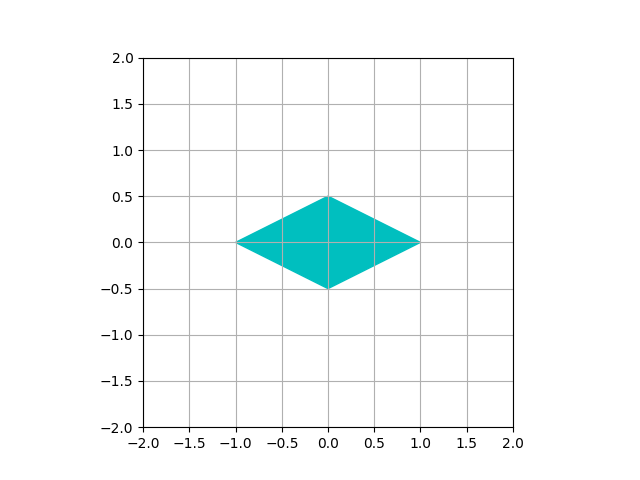
\includegraphics[width=1\linewidth]{pic/orig.png}}
\caption{Оригинал.}
\end{figure}

\newpage
\subsection{Для отображения 1}
\begin{equation}
A =
\begin{bmatrix}
-0.6 & 0.8\\
0.8 & 0.6
\end{bmatrix}
\end{equation}

\begin{figure}[h]
\center{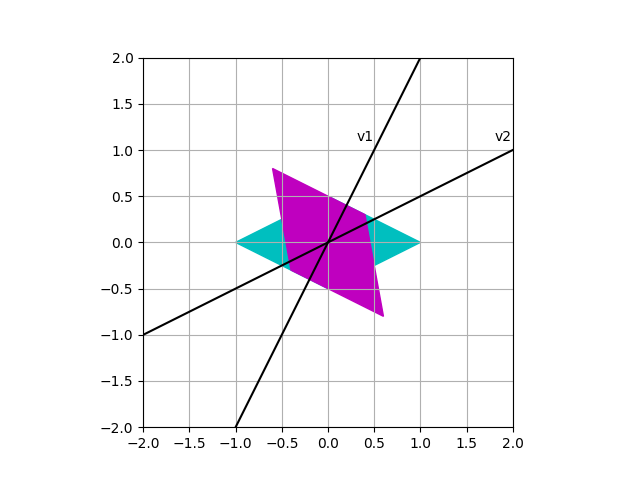
\includegraphics[width=1\linewidth]{pic/1.png}}
\caption{Образ 1 (фиолетовый), оригинал (голубой) и прямые, совпадающие с направлениями собственных векторов.}
\end{figure}


\newpage
\subsection{Для отображения 2}
\begin{equation}
B =
\begin{bmatrix}
1 & 0\\
8 & 0
\end{bmatrix}
\end{equation}

\begin{figure}[h]
\center{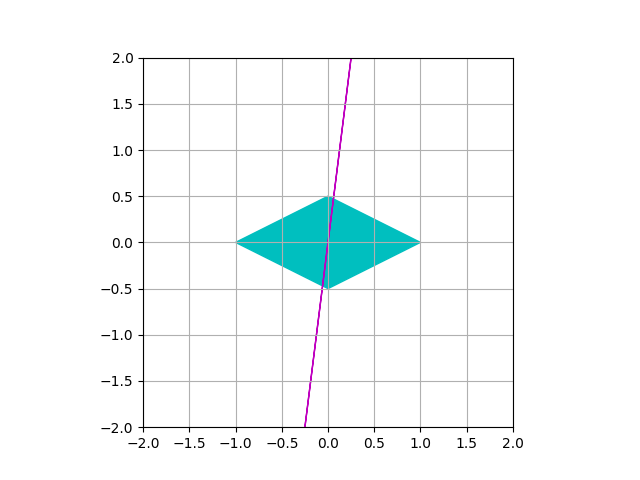
\includegraphics[width=1\linewidth]{pic/2.png}}
\caption{Образ 2 (фиолетовый), оригинал (голубой).}
\end{figure}


\newpage
\subsection{Для отображения 3}
\begin{equation}
C =
\begin{bmatrix}
\cos \frac{5\pi}{18} & -\sin \frac{5\pi}{18}\\
\\
\sin \frac{5\pi}{18} & \cos \frac{5\pi}{18}
\end{bmatrix}
\end{equation}

\begin{figure}[h]
\center{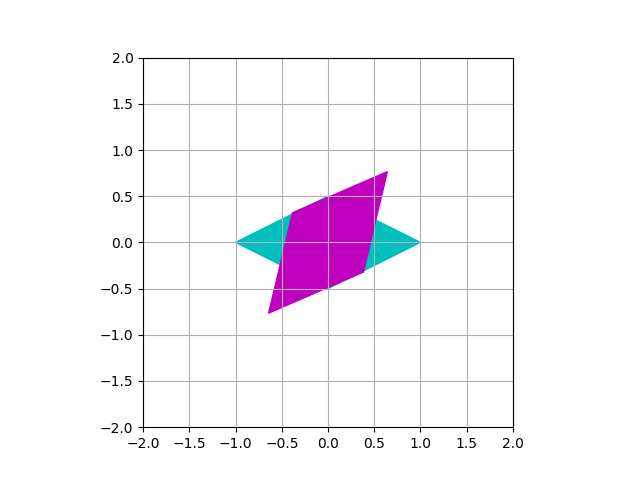
\includegraphics[width=1\linewidth]{pic/3.png}}
\caption{Образ 3 (фиолетовый), оригинал (голубой).}
\end{figure}


\newpage
\subsection{Для отображения 4}
\begin{equation}
D =
\begin{bmatrix}
-1 & 0\\
0 & -1
\end{bmatrix}
\end{equation}

\begin{figure}[h]
\center{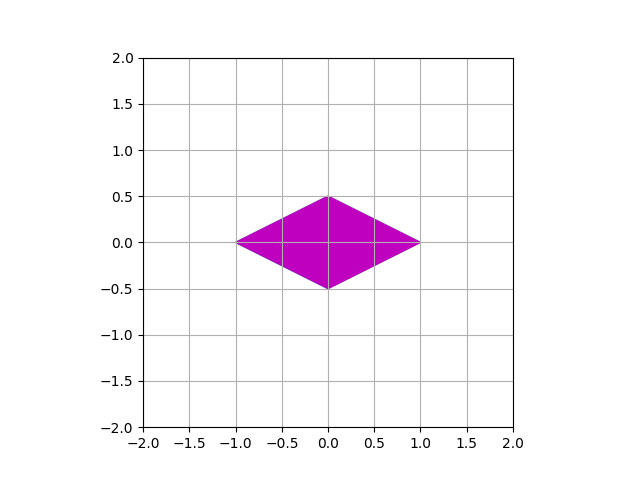
\includegraphics[width=1\linewidth]{pic/4.png}}
\caption{Образ 4 (фиолетовый).}
\end{figure}


\newpage
\subsection{Для отображения 5}
\begin{equation}
F =
\begin{bmatrix}
-0.3\sqrt{3} + 0.4 & 0.4\sqrt{3} + 0.3 \\
0.4\sqrt{3} + 0.3  & 0.3\sqrt{3} - 0.4 
\end{bmatrix}
\end{equation}

\begin{figure}[h]
\center{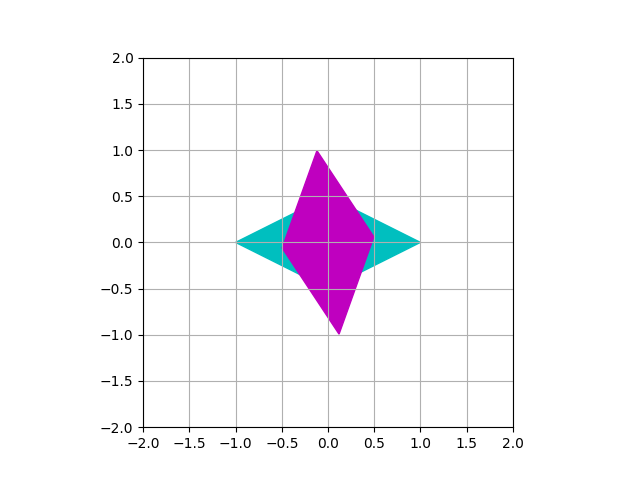
\includegraphics[width=1\linewidth]{pic/5.png}}
\caption{Образ 5 (фиолетовый), оригинал (голубой).}
\end{figure}

\newpage
\subsection{Для отображения 6}
\begin{equation}
G =
\begin{bmatrix}
1 & \frac{1}{8}\\
0 & 1
\end{bmatrix}
\end{equation}

\begin{figure}[h]
\center{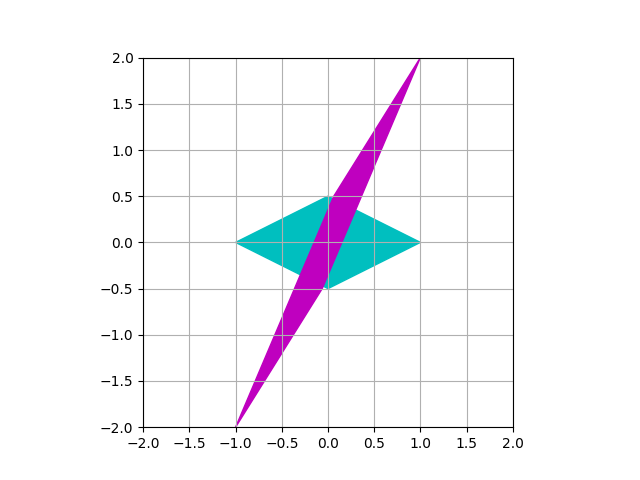
\includegraphics[width=1\linewidth]{pic/6.png}}
\caption{Образ 6 (фиолетовый), оригинал (голубой).}
\end{figure}

\newpage
\subsection{Для отображения 7}
\begin{equation}
H =
\begin{bmatrix}
\frac{4}{3} & - \frac{1}{6}\\
\\
- \frac{8}{3} &  \frac{4}{3}
\end{bmatrix}
\end{equation}

\begin{figure}[h]
\center{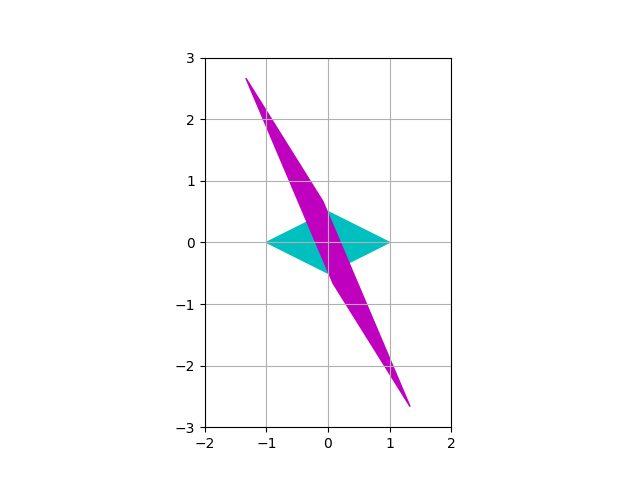
\includegraphics[width=1\linewidth]{pic/7.png}}
\caption{Образ 7 (фиолетовый), оригинал (голубой).}
\end{figure}

\newpage
\subsection{Для отображения 8}
\begin{equation}
K =
\begin{bmatrix}
1 & 0\\
10 & -1
\end{bmatrix}
\end{equation}

\begin{figure}[h]
\center{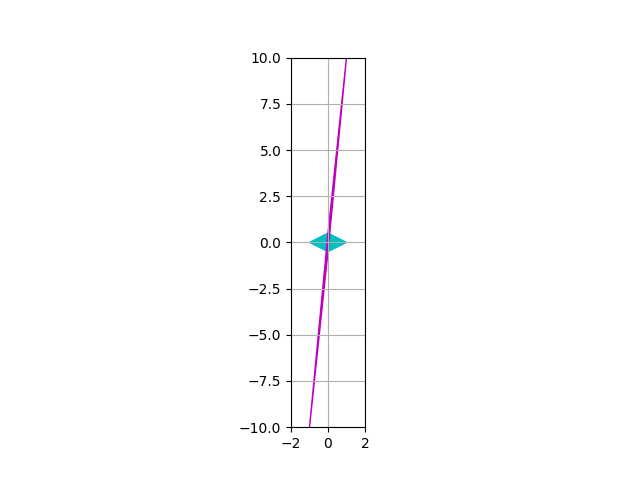
\includegraphics[width=1\linewidth]{pic/8.png}}
\caption{Образ 8 (фиолетовый), оригинал (голубой).}
\end{figure}

\newpage
\subsection{Для отображения 9}
\begin{equation}
L =
\begin{bmatrix}
\sqrt{5} & 0\\
0 & \sqrt{5}
\end{bmatrix}
\end{equation}

\begin{figure}[h]
\center{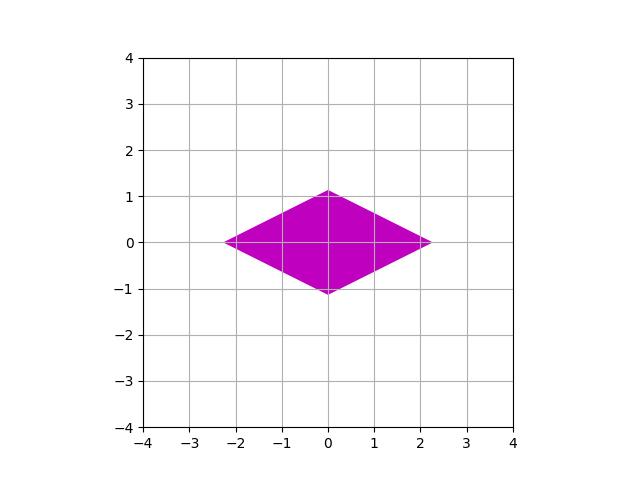
\includegraphics[width=1\linewidth]{pic/9.png}}
\caption{Образ 9 (фиолетовый).}
\end{figure}

\newpage
\subsection{Для отображения 10}
\begin{equation}
M =
\begin{bmatrix}
3 & 0\\
0 & 1
\end{bmatrix}
\end{equation}

\begin{figure}[h]
\center{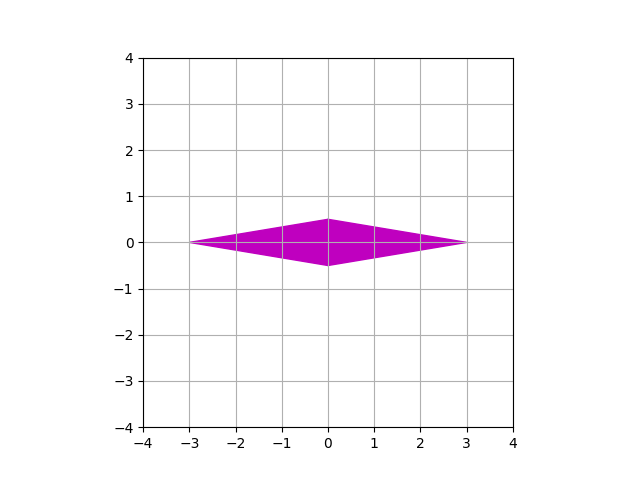
\includegraphics[width=1\linewidth]{pic/10.png}}
\caption{Образ 10 (фиолетовый).}
\end{figure}

\newpage
\subsection{Для отображения 11}
\begin{equation}
N =
\begin{bmatrix}
\frac{6}{5} & \frac{2}{5}\\
\frac{2}{5} & \frac{9}{5}
\end{bmatrix}
\end{equation}

\begin{figure}[h]
\center{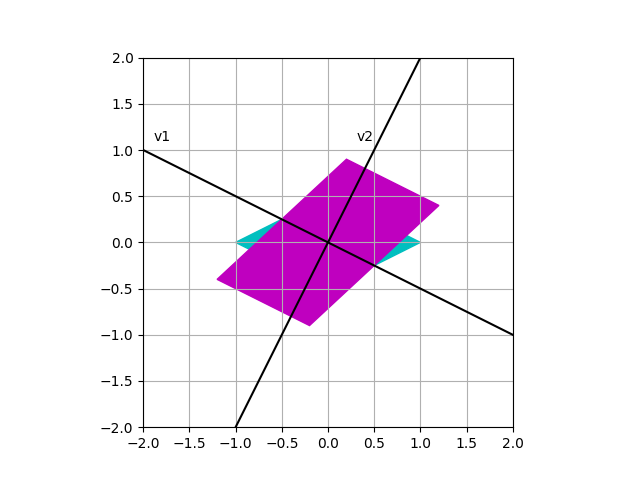
\includegraphics[width=1\linewidth]{pic/11.png}}
\caption{Образ 11 (фиолетовый), оригинал (голубой) и прямые, совпадающие с направлениями собственных векторов.}
\end{figure}

\newpage
\subsection{Для отображения 12}
\begin{equation}
O =
\begin{bmatrix}
4 & 1\\
0 & 4
\end{bmatrix}
\end{equation}

\begin{figure}[h]
\center{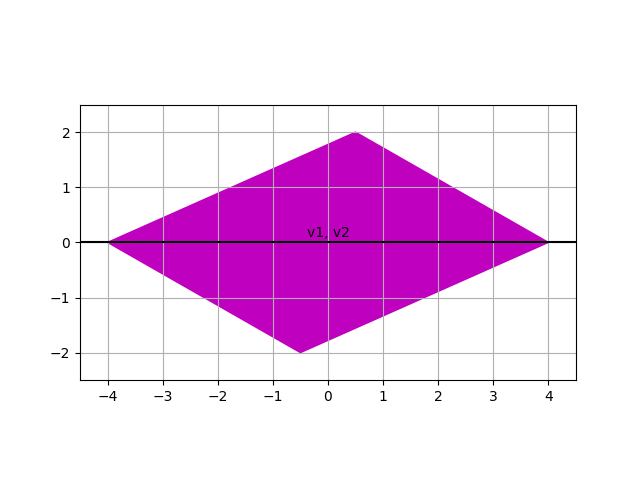
\includegraphics[width=1\linewidth]{pic/12.png}}
\caption{Образ 12 (фиолетовый) и прямые, совпадающие с направлениями собственных векторов.}
\end{figure}


\newpage
\subsection{Для отображения 13}
\begin{equation}
P =
\begin{bmatrix}
0 & -1\\
4 & 0
\end{bmatrix}
\end{equation}

\begin{figure}[h]
\center{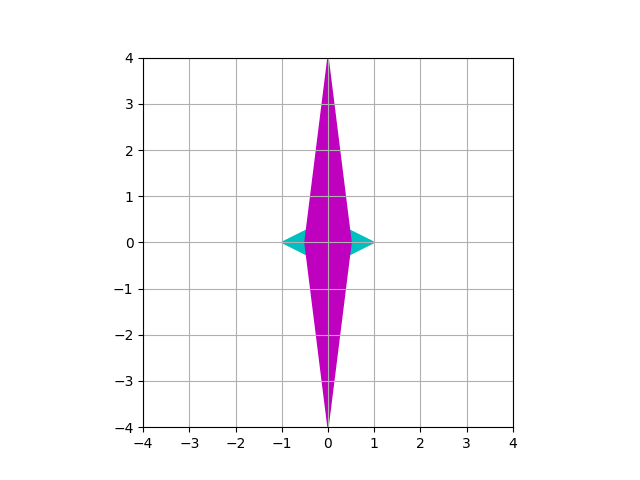
\includegraphics[width=1\linewidth]{pic/13.png}}
\caption{Образ 13 (фиолетовый), оригинал (голубой).}
\end{figure}


\newpage
\subsection{Для отображения 14}
\begin{equation}
Q =
\begin{bmatrix}
0 & 0\\
0 & 0
\end{bmatrix}
\end{equation}

\begin{figure}[h]
\center{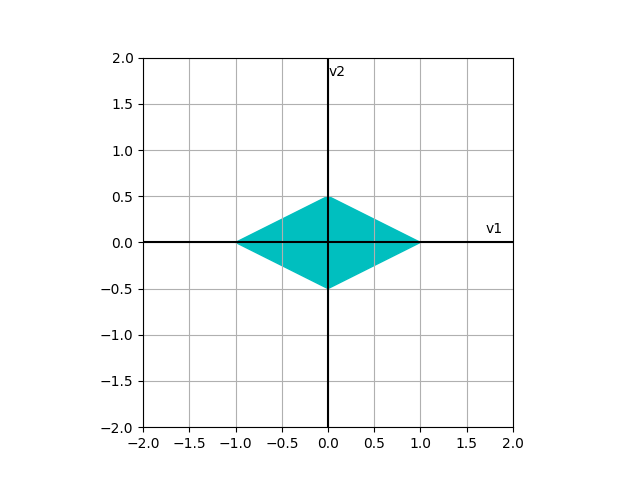
\includegraphics[width=1\linewidth]{pic/14.png}}
\caption{Образ 14 (точка (0, 0)), оригинал (голубой) и прямые, совпадающие с направлениями собственных векторов.}
\end{figure}

\newpage
\subsection{Для отображения 15}
\begin{equation}
S_1 =
\begin{bmatrix}
1 & 2\\
3 & 4
\end{bmatrix}
, \, \, 
S_2 =
\begin{bmatrix}
5 & 6\\
7 & 8
\end{bmatrix}
\end{equation}

\begin{figure}[h!]
\center{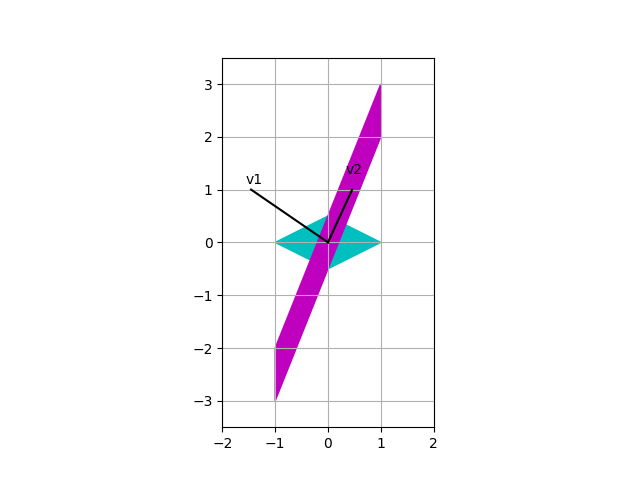
\includegraphics[width=1\linewidth]{pic/15_a.png}}
\caption{Образ 15 для матрицы $S_1$ (фиолетовый), оригинал (голубой) и прямые, совпадающие с направлениями собственных векторов.}
\end{figure}

\newpage
\begin{figure}[h!]
\center{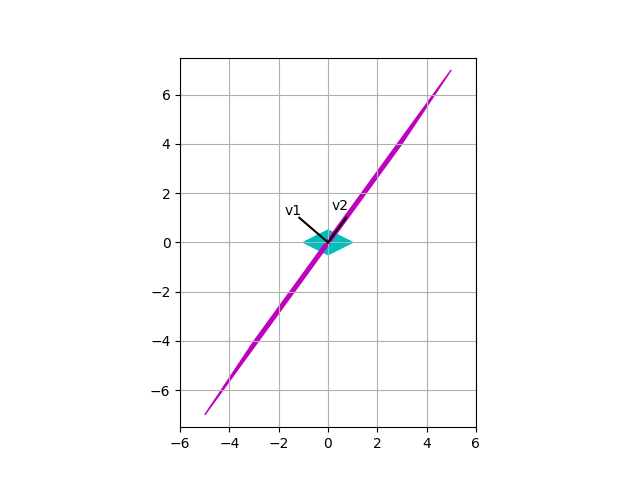
\includegraphics[width=1\linewidth]{pic/15_b.png}}
\caption{Образ 15 для матрицы $S_2$ (фиолетовый), оригинал (голубой) и прямые, совпадающие с направлениями собственных векторов.}
\end{figure}

\newpage
\begin{figure}[h!]
\center{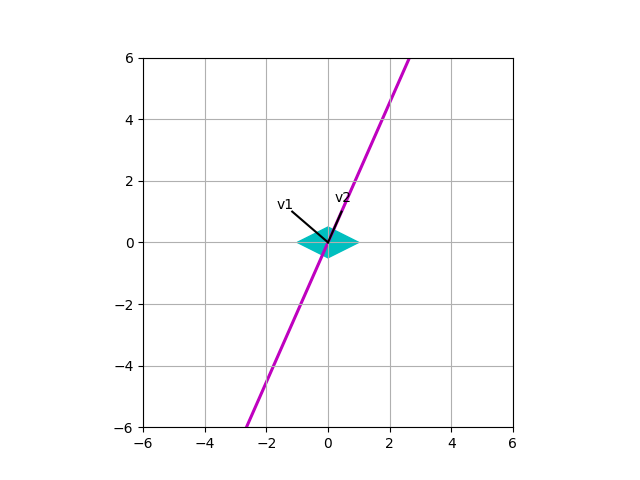
\includegraphics[width=1\linewidth]{pic/15_ab.png}}
\caption{Образ 15 для матрицы $S_1 S_2$ (фиолетовый), оригинал (голубой) и прямые, совпадающие с направлениями собственных векторов.}
\end{figure}

\newpage
\begin{figure}[h!]
\center{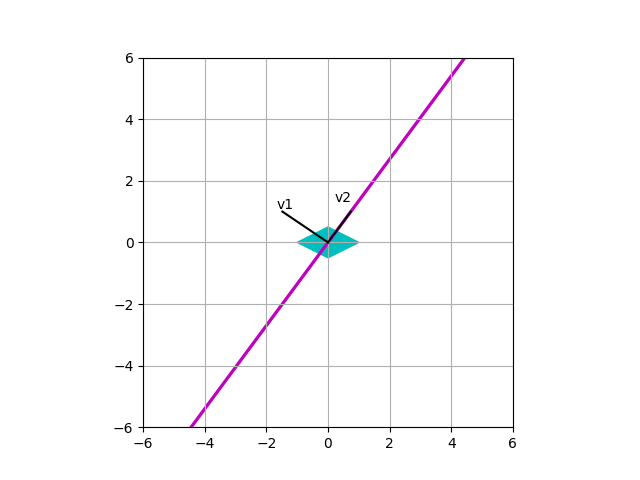
\includegraphics[width=1\linewidth]{pic/15_ba.png}}
\caption{Образ 15 для матрицы $S_2 S_1$ (фиолетовый), оригинал (голубой) и прямые, совпадающие с направлениями собственных векторов.}
\end{figure}

\newpage
\subsection{Для отображения 16}
\begin{equation}
T_1 =
\begin{bmatrix}
1 & 4\\
0 & 2
\end{bmatrix}
, \, \, 
T_2 =
\begin{bmatrix}
9 & 8\\
0 & 11
\end{bmatrix}
\end{equation}

\begin{figure}[h]
\center{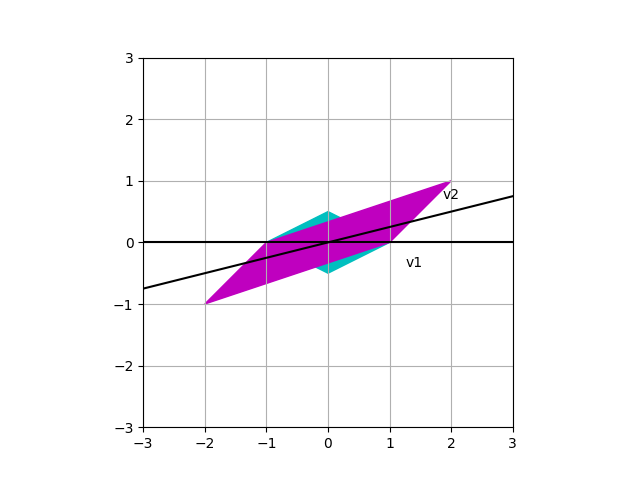
\includegraphics[width=1\linewidth]{pic/16_a.png}}
\caption{Образ 16 для матрицы $T_1$ (фиолетовый), оригинал (голубой) и прямые, совпадающие с направлениями собственных векторов.}
\end{figure}


\newpage
\begin{figure}[h!]
\center{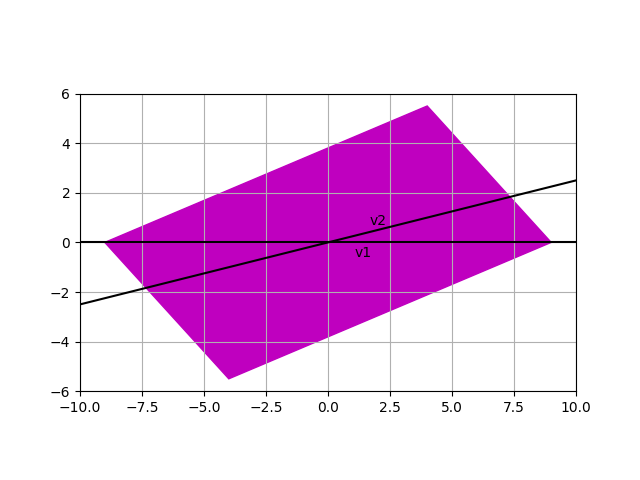
\includegraphics[width=1\linewidth]{pic/16_b.png}}
\caption{Образ 16 для матрицы $T_2$ (фиолетовый), оригинал (голубой) и прямые, совпадающие с направлениями собственных векторов.}
\end{figure}

\newpage
\begin{figure}[h!]
\center{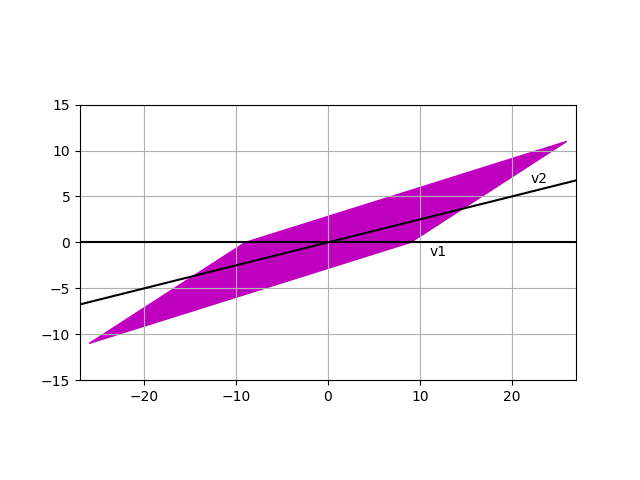
\includegraphics[width=1\linewidth]{pic/16_ab.png}}
\caption{Образ 16 для матрицы $T_1 T_2$ (фиолетовый), оригинал (голубой) и прямые, совпадающие с направлениями собственных векторов.}
\end{figure}

\newpage
\begin{figure}[h!]
\center{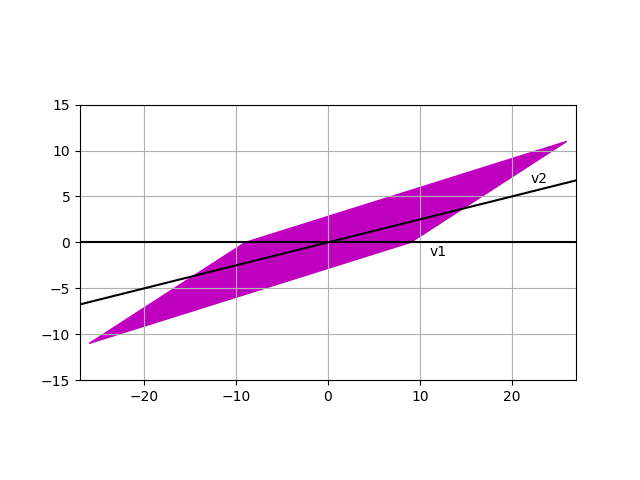
\includegraphics[width=1\linewidth]{pic/16_ba.png}}
\caption{Образ 16 для матрицы $T_2 T_1$ (фиолетовый), оригинал (голубой) и прямые, совпадающие с направлениями собственных векторов.}
\end{figure}


\end{document}













